\section{Lektion 08-02-2018}

\begin{enumerate}
	\item Måling af lydtryk
	\item Mikrofon
	\item Udstyr til lydmåling
	\item Måleprincipper
\end{enumerate}

\noindent\fbox{\parbox{\textwidth}{
\begin{itemize}
	\item \textbf{Pensum:} 
	\begin{enumerate}
		\item Audio Meetering, sec. 8-9, 26-29
		\item Elektroakustik, TAS,  p. 12-14
	\end{enumerate}
	\item \textbf{Opgaver:} 
	\begin{enumerate}
		\item Lyd og Akustik - Lektion 2 - opgaver og øvelser
	\end{enumerate}
\end{itemize}
}} \vspace{3mm}

\subsection{Måling af lydtryk}
\begin{itemize}
	\item Et reference lydtryk er valgt til at være \SI{20}{\micro\pascal} hvilket svarer til den mindste ændring i tryk et menneske kan opfange.
	\item Forholdet mellem det statiske tryk og reference lydtrykket er $1 :
	5.066.250.000$.
	\begin{itemize}
		\item Lydtryk (sound pressure),  Pascal [\si{\pascal}]
		\item Lydtrykniveau (sound pressure level - SPL), Decibel [\si{\decibel}]
	\end{itemize}
\end{itemize}

\begin{itemize}
	\item Lydstyrke udtrykt som lydtrykniveau [\si{\decibel}] i stedet for lydtryk [\si{\pascal}]
\end{itemize}

\begin{equation}\label{eq:spl1}
SPL = 20\log_{10}\left(\frac{p}{p_{ref}}\right)
\end{equation}

\begin{itemize}
	\item $SPL$ = sound pressure level, \si{\decibel}
	\item $p$ = acoustic pressure, \si{\micro\pascal}
	\item $p_{ref}$ = acoustic reference pressure, \SI{20}{\micro\pascal}.
\end{itemize}

\subsection{Mikrofon}
\begin{itemize}
	\item En transducer der omsætter et oscillerende lydtryk til et analogt elektrisk signal.
	\begin{itemize}
		\item Kaldes også for en tryktransducer.
		\item Måler lydtrykkets variation i et punkt uden reference til den retning lyden udbredes i.
		\item Flere mikrofontyper er retningsbestemte på grund af deres opbygning.
	\end{itemize}
	\item Mikrofoner – 4 hovedgrupper
	\begin{itemize}
		\item Studiemikrofoner (Dynamiske- og kondensator mikrofoner)
		\item Målemikrofoner (Kondensator mikrofoner)
		\item Mikrofonkapsler (Elektret mikrofoner)
		\item MEMS mikrofoner (Silicium mikrofoner)
	\end{itemize}
\end{itemize}

\subsubsection{Dynamisk mikrofon}
\begin{itemize}
	\item \textbf{Klassiske form}: minder om en højttaler (membranen sættes i bevægelse af lydtrykket). Derved bevæges svingspolen i magnetfeltet
	og der induceres en spænding.
	\item \textbf{Båndmikrofonen}: membranen er i et kraftigt magnetfelt. Når lydtrykket får membranen til at svinge induceres der en spænding over de to ender af båndet. Spændingen er normalt så lav at der skal benyttes en transformator for at løfte det op på et brugbart niveau. 
	\begin{itemize}
		\item Lyden har adgang til begge sider af membranen.
		\begin{itemize}
			\item Mest følsom for lyd på aksen ($0\degree$ og $180\degree$.
			\item Der kan ikke registreres lyd fra siden ($90\degree$).
		\end{itemize}
	\end{itemize} 
\end{itemize}
\begin{figure} [H]
	\centering
	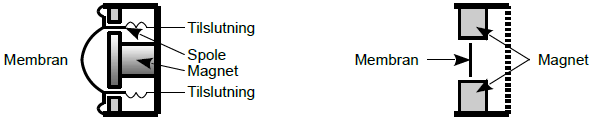
\includegraphics[width=.85\linewidth]{graphics/12.png}
	\caption{V: svingspolen drives af en membran til at svinge i et magnetfelt. H: En tynd metalfolie svinger i et magnetfelt.}
	\label{fig:12}
\end{figure}

\begin{itemize}
	\item Beregnet til optagelser af musik og sang.
	\item Ikke forberedt til at blive kalibreret.
	\item Frekvensrespons er designet til at lyde "godt", "fedt" eller "spændende".
	\item Fysisk størrelse er ikke vigtig (forskellige designs afhængig af brand).
	\item Typisk lavt støjniveau pga. stor membran diameter.
	\item Ikke velegnet til akustiske målinger.
\end{itemize}

\subsubsection{Kondensator mikrofon}
\begin{itemize}
	\item En tynd membran af udspændt metalfolie er anbragt tæt på
	en fastsiddende elektrode.
	\item Kondensatoren mellem membran og elektrode oplades gennem $R_p$. 
	\item Spændingen mellem membran og elektrode vil variere efter definitionsligningen $Q = C\cdot U$.
	\begin{itemize}
		\item $Q$ er den konstante ladning givet af polarisationsspændingen $U_P$ der ved målemikrofoner typisk er \SI{200}{\volt}.
	\end{itemize}
	\item Den lave grænsefrekvens sættes af $R_p$ og mikrofonens kapacitet $C$.
	\begin{itemize}
		\item $C \approx \SI{5}{\pico\farad}-\SI{20}{\pico\farad}$ gør at  $R_p$ skal være mindst \SI{1}{\giga\ohm} for måling af hørbar lyd.
	\end{itemize}
	\item Den høje grænsefrekvens sættes af membranens masse. 
\end{itemize}

\begin{figure} [H]
	\centering
	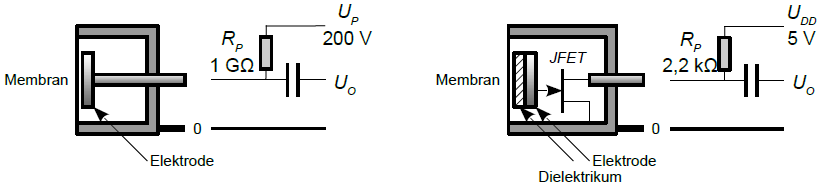
\includegraphics[width=.85\linewidth]{graphics/11.png}
	\caption{Kondensatormikrofons opbygning.}
	\label{fig:11}
\end{figure}

\begin{itemize}
	\item Alternativt indbygges en plastskive mellem membran og elektrode hvor en såkaldt "fastfrosset ladning" fungerer som $Q$.
	\item Den høje udgangsimpedans sænkes af en indbygget JFET og det eksterne kredsløb skal nu levere strøm til transistorens drain.
	\item Beregnet til til akustiske målinger da "alle" specifikationer er kendte.
	\item Generelt er der to typer: "Frit-felts kalibrede" og "Tryk-felts kalibrerede".
	\item Tager højde for at den måde mikrofonen selv forstyrrer lydfeltet på.
	\item Stor diameter vælges til lave frekvenser og lave lydtryk.
	\item Lille diameter vælges til høje frekvenser og høje lydtryk.
\end{itemize}

\subsubsection{Elektretmikrofoner}
\begin{itemize}
	\item Mikrofonkapsler.
	\item Velegnet til mange forskellige formål – også målinger selvom få specifikationer er kendte.
	\item Prisen er meget attraktiv: 1-2 \$
	\item Ingen forskel på "Frit-felt" og "Tryk-felt" grundet lille membran-åbning.
	\item Vælg mellem kommunikations mikrofoner og bredbåndet mikrofon.
	\item Som regel 6-10 \si{\milli\meter} diameter.
	\item Benytter 2-10 VDC strømforsyning.
	\item Kvaliteten afhænger meget af forstærker og strømforsyning.
\end{itemize}

\subsubsection{MEMS mikrofoner}
\begin{itemize}
	\item Silicium mikrofoner.
\end{itemize}

\subsection{Mikrofon for-forstærkere}
\begin{itemize}
	\item LM337/LM137, 3-Terminal Adjustable Regulators
	\begin{itemize}
		\item Justerbar $V_{out}$.
		\item 1/3 støj på $V_{out}$.
		\begin{itemize}
			\item Overvej en 2-trinsregulering (1/3 af 1/3 støj).
		\end{itemize}
	\end{itemize}
	\item LM8333/OP27, Audio Operational Amplifier
	\begin{itemize}
		\item Made for audio purpose.
		\item Specified low noise voltage.
	\end{itemize}
\end{itemize}

\subsection{Udstyr til lydmåling}
\begin{itemize}
	\item Pistonfon
	\item \textbf{Lydtrykkalibrator}
	\item Elektrostatisk aktuator
	\item Reciprocitets kalibrering
\end{itemize}

\subsubsection{Pistonfon}
\begin{itemize}
	\item Frembringer et meget veldefineret lydtryk i et lille kammer.
	\item Ind i åbningen stikkes mikrofonen, som herved påvirkes med et kendt lydtryk.
	\begin{itemize}
		\item Lydtrykniveau: \SI{124}{\decibel}
		\item Tolerance: $\pm$\SI{0.2}{\decibel}
		\item Testfrekvens: \SI{250}{\hertz}
	\end{itemize}
\end{itemize}

\begin{figure} [H]
	\centering
	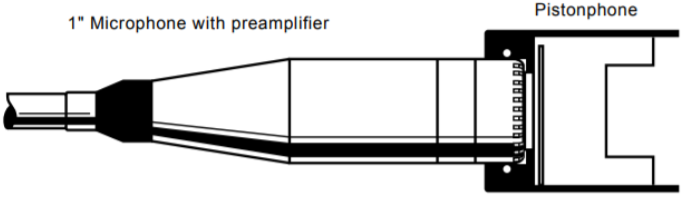
\includegraphics[width=\linewidth]{graphics/2.png}
	\caption{Pistonfon.}
	\label{fig:2}
\end{figure}

\subsubsection{Lydtrykkalibrator}
\begin{itemize}
	\item Lydtrykniveau: \SI{94}{\decibel} eller \SI{114}{\decibel}
	\item Tolerance: $\pm$\SI{0.3}{\decibel}
	\item Testfrekvens: \SI{1000}{\hertz}
\end{itemize}

\subsubsection{Elektrostatisk Aktuator}
\begin{itemize}
	\item Lydtrykniveau: \SI{70}{\decibel} - \SI{90}{\decibel}
	\item Tolerance: $\pm$\SI{0.5}{\decibel}
	\item Testfrekvens: \SI{1.0}{\kilo\hertz}-\SI{40.0}{\kilo\hertz}
\end{itemize}

\subsubsection{PC-baseret udstyr til lydmåling}
\begin{itemize}
	\item TrueRTA.com
	\item YMEC.com
\end{itemize}

\subsection{Måleprincipper}
\subsubsection{Frekvensanalyse}
\begin{itemize}
	\item Stepped sinus
	\item Sinus sweep
	\item Oktavbåndsanalyse (Constant Percentage Bandwidth - CPB)
	\item Fast Fourier Transform (FFT)
\end{itemize}

\subsubsection{Impulsresponser og overføringsfunktioner}
\begin{itemize}
	\item En impulsrespons eller overføringsfunktion kan fuldstændig beskrive et LTI-system (Lineært og	Tidsinvariant).
	\item Disse responser kan bestemmes ved at tilføje et velegnet input-signal til systemet og derefter samtidig betragte input, x[n] og output, y[n].
	\item Med krydskorrelation kan vi bestemme impulsresponsen (xcorr i matlab)
	\newpage\item Et velegnet input signal kan være:
	\begin{itemize}
		\item Random Noise
		\item MLS (maximum length sequence)
		\begin{itemize}
			\item Sekvensen repeteres efter ($2\cdot N-1$) samples for et N'
			te ordens skifteregister.
			\item Output amplitude er binary [$-1; 1$].
			\item Output er 'pseudo random' hvid støj.
			\item Auto-correlation er næsten perfekt.
			\item Sekvens længden vil altid være et radix-2 antal af samples samples -1.
			\item Dækker hele frekvensintervallet fra \SI{0}{\hertz} til $\frac{f_s}{2}$.
		\end{itemize}
	\end{itemize}
\end{itemize}

\begin{figure} [H]
	\centering
	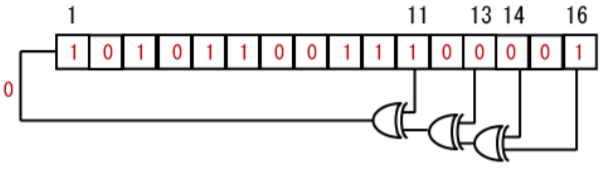
\includegraphics[width=0.6\linewidth]{graphics/45.png}
	\caption{MLS sekvens.}
	\label{fig:45}
\end{figure}

\begin{itemize}
	\item[] 
	\begin{itemize}
		\item Logaritmisk sinus sweep
		\begin{itemize}
			\item Output har konstant amplitude.
			\item Auto-correlation er god.
			\item Sekvensens længde kan vælges arbitrært men bestemmer måletiden.
			\item Fantastisk udnyttelse af dynamic området (højt signal-støj forhold, SNR).
			\item Sweeps kan bade være stigende og faldende i frekvens.
			\item Dækker frekvensområdet [$f_1 – f_2$].
		\end{itemize}
	\end{itemize}
\end{itemize}

\begin{equation}
x(t)=\sin \left[\dfrac{2\pi f_1 T}{\ln
	\left(\frac{f_2}{f_1}\right)}\left(e^{\frac{t}{T}\ln
	\left(\frac{f_2}{f_1}\right)}-1\right)\right]
\end{equation}

\newpage
\begin{itemize}
	\item Matematiske funktioner for sekvenser
	\begin{itemize}
		\item \textbf{Filtrering}
		\begin{itemize}
			\item Convolution $(f\circledast g)(t) = \int_{-\infty}^{\infty}f(\tau)g(t-\tau)d\tau$ 
			\item[]
		\end{itemize}
		\item \textbf{Mønstergenkendelse}
		\begin{itemize}
			\item Cross-corelation $(f\star g)(t) =\int_{-\infty}^{\infty}f*(\tau)g(t+\tau)d\tau$
			\item[]
		\end{itemize}
		\item \textbf{Gentagelsesgrad}
		\begin{itemize}
		\item Auto-correlation $(f\star f)(t) =\int_{-\infty}^{\infty}f*(\tau)f(t+\tau)d\tau$
		\item[]
		\end{itemize}
	\end{itemize}
	\item En lang måletid giver mere præcise resultater end korte måletider.
	\begin{itemize}
		\item Hver gang man fordobler antallet af målinger (repetitioner) kan SNR forbedres med \SI{6}{\decibel} ved midling.
	\end{itemize}
	\item De mest præcise resultater for konstant måletid er "Logaritmisk Sinus
	Sweep".
\end{itemize}
